\chapter{Management von Risiken bei Anmeldesystemen}
\strahlhofer

%Systemplanung und Projekte Entwicklung von Felix Schwab, Ingridschwab-Matkovits
%https://searchcompliance.techtarget.com/definition/risk-management#:~:text=Risk%20management%20is%20the%20process,errors%2C%20accidents%20and%20natural%20disasters.
\section{Risikomanagement im Bereich Anmeldesysteme}
Das Risikomanagement muss für jedes Unternehmen eine Top-Priorität sein. Durch dieses Verfahren können zukünftige Bedrohungen abgeschätzt und sich dazu Bewältigungsstrategien überlegt werden. Eine Firma muss sich im Vorhinein überlegen welche Risiken eintreten können. Diese Bedrohungen können durch viele verschiedene Ereignisse, wie z.B. durch Naturkatastrophen, rechtliche Verpflichtungen, Managementfehler und sonstige Unfälle eintreten.
Mit der Planung einer neuen oder ausbaubaren IT-Infrastruktur sollte unbedingt das Risikomanagement in Betracht gezogen werden. Die Firma muss versuchen Risiken zu vermeiden oder diese bis zu einem gewissen Grad zu vermindern\footcite{risikomanagement-diplomarbeit}\footcite{risikomanagement}. 

\begin{center}
\begin{figure}[H]
    \centering
    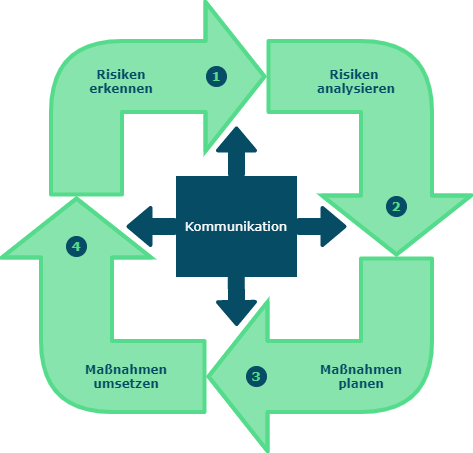
\includegraphics[width=9cm]{Risikomanagement_zyklus.png}
    \caption{Ablauf des Risikomanagements (in Anlehnung auf die Darstellung des BVA)}
\end{figure}
\end{center}


\section{Grundbegriffe Risikomanagement}
%Systemplanung und Projekte Entwicklung von Felix Schwab, Ingridschwab-Matkovits
\subsection{Risiko}
Unter dem Begriff Risiko assoziiert man im Bereich IT-Sicherheit die Schadenshöhe, wenn ein bestimmtes Ereignis eintritt. Diese Ereignisse haben einen negativen Effekt auf das Unternehmen. Sie tragen dazu bei, dass materielle oder immaterielle Schäden auftreten können oder sogar Arbeitsprozesse abstoppen\footcite{risikomanagement-diplomarbeit}.

%Systemplanung und Projekte Entwicklung von Felix Schwab, Ingridschwab-Matkovits
\subsection{Maßnahme}
Eine Maßnahme ist eine Handlung, die ermöglicht ein Risiko zu umgehen oder es einzugrenzen. Hier spricht wird von einer Schadensminimierung gesprochen\footcite{risikomanagement-diplomarbeit}. 

%https://www.bva.bund.de/DE/Services/Behoerden/Beratung/Beratungszentrum/GrossPM/s-o-s_handbuch/stda_sos-kap8_risikomgmt.html
\section{Ziele des Risikomanagements}
Die Ziele, die ein Unternehmen im Blick haben muss sind:
\begin{enumerate}
	\item \textbf{Risiken ausführlich identifizieren:} Die Firma darf keinesfalls essentielle Risiken übersehen.
	\item \textbf{Risiken geeignet bewerten:} Bedrohungen / Risiken sollen in Hinsicht auf die Eintrittswahrscheinlichkeit, mögliche Auswirkungen und auf zeitliche Nähe eingeschätzt werden. Zusätzlich sollen diese darauffolgend mit dieser Betrachtungsweise bewertet werden.
	\item \textbf{Gleichgewicht zwischen Analyse und Umsetzung:} Hier wird versucht eine Balance zwischen Risiken analysieren und dem Auftraggeber und der Projektleitung diese aufzuzeigen zu finden. Zum anderen muss beachtet werden, das Gegenmaßnahmen getroffen werden.
	\item \textbf{Minimierung von Risiken:} Ein Risiko an sich, kann nicht verändert werden. Das Unternehmen kann lediglich durch ein aktives entgegenwirken, die Wahrscheinlichkeit des Eintretens vermindern oder verhindern.
	\item \textbf{Kommunikation:} Dieses Ziel gibt an das die Risiken dem Auftraggeber rechtzeitig übermittelt werden.
	\item \textbf{Überwachung:} Alle diese Ziele müssen für neue oder schon bekannte Risiken immer wieder zyklisch durchgeführt werden\footcite{bva-risikomanagement}. 
\end{enumerate}

\section{Umsetzungsprozesse}
Im Risikomanagement existieren grundsätzlich zwei Arten von Umsetzungsprozessen. Diese unterscheidet man in initiale Prozesse und laufende Prozesse.
Diese beiden Prozesse werden auch als Aufbau Risikomanagement bezeichnet, da alle Vorkehrungen im Vorhinein eines Projekts getätigt werden und als laufendes Risikomanagement, da dieses während der Durchführung des Projekts durchgeführt wird, bezeichnet\footcite{bva-risikomanagement}.

\section{Aufbau Risikomanagement}
\subsection{Verantwortungszuweisung und Budgetierung}
Bei der Aufbereitung des Risikomanagements müssen am Anfang die Rollen jeder einzelnen Person, die Einfluss auf das Projekt besitzt, festgelegt werden. Es werden alle Stakeholder erfasst. Das sind Personen die einen Einfluss auf das Projekt besitzen.
Zusätzlich muss ein Budget festgelegt werden, welches für die Bewältigung eines Risikos eingesetzt wird. Hier muss gegenübergestellt werden wie viel Kosten entstehen, falls das Risiko eintritt und wie viel in diesem Fall die Bewältigung kostet\footcite{bva-risikomanagement}.

%https://www.business-wissen.de/hb/risiken-identifizieren/#:~:text=Insofern%20ist%20die%20Identifikation%20von,Sch%C3%A4den%20unvorhergesehen%20und%20%C3%BCberraschend%20eintreten.
\subsection{Risikoidentifikation}
Alle Risiken zu identifizieren, die möglicherweise auftreten können, kann sich als sehr schwer erweisen. Es können etwaige Risiken auftreten, von denen noch nichts bekannt war oder die man nicht in Betracht gezogen hat. Aus diesen Gründen spielt die Identifikationsphase eine sehr wichtige Rolle. Sie muss sorgfältig durchgeführt werden und mit verschiedenen Ansätzen abgewickelt werden. Fortlaufend sollte deswegen regelmäßig überprüft werden, ob sich Risiken verändern oder möglicherweise hinzukommen\footcite{risikoidentifikation-definition}.

%Methoden gefunden: Im Syp Buch
%https://de.wikipedia.org/wiki/Risikoidentifikation#:~:text=Als%20Methoden%20kommen%20f%C3%BCr%20bestehende,oder%20die%20Delphi%2DMethode%20ermitteln.
\subsubsection{Bestehende Risiken und Potenzielle Risiken}
Die Risikoidentifikation beschäftigt sich mit zwei Arten von Risiken auf der einen Hand mit den bekannten Risiken, auf der anderen potenziellen Risiken. Folgende Methoden können zur Bewältigung angewandt werden:
\begin{enumerate}
    \item \textbf{Methoden um bestehende/bekannte Risiken zu identifizieren}
    \begin{itemize}
        \item Einsatz von Checklisten
        \item SWOT-Analyse
        \item Befragungen von erfahrenen Mitarbeitern
        \item Befragungen von Experten mit spezifischen Fachwissen
    \end{itemize}
    \item \textbf{Methoden um Potenzielle Risiken zu identifizieren}
    \begin{itemize}
    	\item Brainstorming
    	\item Brainwriting (bzw. 6-3-5 Methode)
    	\item Delphi-Methode
    	\item Mindmapping
    	\item Morphologischer Kasten
    \end{itemize}
\end{enumerate}

%https://de.wikipedia.org/wiki/Risikoidentifikation#Checklisten_und_Mitarbeiterbefragungen
\subsubsection{Einsatz von Checklisten}
Bei dieser Methode werden standardisierte Checklisten verwendet. Diese sollen einem Unternehmen aufzeigen welche Risiken zu beachten sind, wenn es um die Informationssicherheit geht. Hier besteht jedoch ein Nachteil, denn es werden nicht alle für das eigene Unternehmen relevanten Risiken genannt.

%https://smallbusiness.chron.com/security-swot-analysis-40526.html
\subsubsection{SWOT-Analyse}
SWOT(Strengths, Weaknesses, Opportunities, Threats) ist eine Methode verschiedene Faktoren zu analysieren. 
Durch die Infragestellung stellen der Stärken (Strengths) und der Schwächen (Weaknesses) einer Firma können unternehmensinterne Faktoren identifiziert werden.
Durch Hinterfragen von Möglichkeiten (Opportunities) und Bedrohungen (Threats) werden externe Faktoren gefunden, die mit einfließen.


%https://de.wikipedia.org/wiki/Risikoidentifikation#Checklisten_und_Mitarbeiterbefragungen
\subsubsection{Befragungen}
Bei diesen Umfragen werden entweder erfahrene Mitarbeiter oder Experten mit gewissen Fachkompetenzen befragt. Der Vorteil bei der Befragung von Mitarbeitern ist, dass sie eher interne Unternehmensrisiken identifizieren. Bei dem Einsatz von Experten werden eher externe für das Unternehmen bedrohliche Risiken erkannt. Befragungen können in einer digitalen, schriftlichen oder mündlichen Art stattfinden.
Wichtig ist es bei diesen Befragungen, dass die Fragen genau zu beschreiben und sie sinnvoll auf das Unternehmen anzupassen.

%Buch S. 38
\subsubsection{Brainstorming}
Hier versammeln sich eine Gruppe von unternehmensinternen Personen bestehend aus bevorzugterweise fünf bis sieben Personen. 
Beim Brainstorming-Prozess werden Vorschläge und Ideen nur verbal geäußert und danach dokumentiert. Eine Person, der sogenannte Moderator leitet diesen Kommunikationsprozess. Vorzugsweise sollte dieser Vorgang nur zehn bis maximal zwanzig Minuten andauern.
Die Bewertung der erhobenen Ideen / Vorschlägen darf nicht gleichzeitig mit der Erhebung ablaufen und darf deswegen nur in einer zweiten Phase abgehalten werden. 

Es gibt gewisse Regeln die zu beachten sind:
\begin{itemize}
	\item Keine Barrieren: Das bedeutet, dass eine Person alles vorschlagen kann, auch wenn es eine absurde Idee oder nicht umsetzbar ist. Keine Idee ist zu extrem.
	\item Keine Diskriminierung: Damit ist gemeint, dass kein Teilnehmer für eine geäußerte Idee kritisiert werden soll. Diese Regel ist sehr wichtig, da es sonst den kreativen Prozess stört oder sogar verhindert\footcite{risikomanagement-diplomarbeit-methoden}.
\end{itemize}

%Buch S. 38
\subsubsection{Brainwriting (6-3-5 Methode)}
Bei dieser Methode gibt es sechs Personen, die sich zusammensetzen. Jeder Teilnehmer soll dann jeweils 3 Ideen schriftlich festhalten, in einer Zeit von ungefähr 5 Minuten.
Als nächster Schritt wird dann das Schriftstück in der Runde verteilt. Das kann entweder in eine Richtung weitergegeben werden oder sie werden durchgemischt und dann verteilt. 
Als Ergebnis dieser Methode sollten nach 30 Minuten 108 Ideen aufgeschrieben worden sein.
Der Vorteil dieser Methode ist, dass alle Ideen dokumentiert worden sind und die Ergebnisse deshalb in einer schriftlichen Form vorhanden sind\footcite{risikomanagement-diplomarbeit-methoden}.

%Buch S. 41
\subsubsection{Delphi-Methode}
Bei der Delphi-Methode wird eine Problemstellung oder ein Risiko von einer Gruppe aus verschiedenen und nicht voneinander abhängigen Experten bzw. Fachleuten bearbeitet. 
Jeder Teilnehmer erarbeitet auf einem Schriftstück einen Lösungsansatz, um das gestellte Problem zu lösen.
Die Ausarbeitungen werden eingesammelt und anonymisiert weitergegeben.
Der erhaltene Lösungsansatz soll jetzt kritisiert werden, das heißt falls die Person Denkfehler oder falsche Ansätze verwendet. Aus dieser Bearbeitung soll man für das eigene Konzept Ideen oder Änderungen finden und integrieren.
Dieser Prozess soll mehrere Male wiederholt werden, sodass die Gruppe eine gemeinsame Lösung beschließt.
Die Anonymität spielt bei der Methode eine große Rolle und trägt dazu bei, dass jeder Teilnehmer kreative und alternative Standpunkte einnimmt.
Der Vorteil diese Methode anzuwenden ist, dass unabhängige Fachleute eingesetzt werden und diese über einen größeren Zeitraum an dieser Problematik arbeiten.
Ein daraus folgender Nachteil ist ein hoher Zeit- und Organisationsaufwand\footcite{risikomanagement-diplomarbeit-methoden}.

%buch
\subsubsection{Mindmapping}
Das Mindmapping ist eine Methode, die angewandt wird, um Assoziationen zu einem Thema grafisch darzustellen.
Die Methode ist sehr einfach zu bewältigen und bringt beide Gehirnhälften zum Arbeiten. Die linke Gehirnhälfte die analytische Denkprozesse durchführt und die rechte Hälfte die über den kreativen und intuitiven Teil des Denkens zuständig ist\footcite{risikomanagement-diplomarbeit-methoden}.

%https://de.wikipedia.org/wiki/Assoziation_(Psychologie)
\paragraph{Assoziationen:} 
Eine Assoziation ist in der Psychologie so definiert, das zu einem Thema gewisse Ideen oder Vorstellungen verknüpft werden. Diese Verknüpfungen können durch eine ausgelöste Emotion oder einen bestimmten Sinneseindruck geschaffen werden. Daraus folgen Denkprozesse zu diesem Thema\footcite{assoziationen}. 

%Buchseite 40
\paragraph{Durchführung:}
Es wird ein Thema erfasst und z.B. auf ein Whiteboard oder einen Zettel geschrieben. Dies ist das Zentralthema was von der Gruppe behandelt wird.
Darauffolgend werden gewisse Untersektionen erstellt, diese sollen versuchen das Hauptthema aufzuspalten in kleiner Unterthemenpakete.
Die Teilthemen vom Hauptthema nennt man Hauptäste.
Dieses Aufteilungsverfahren kann so oft wie nötig wiederholt werden, in dem die Themen immer weiter aufgeteilt werden, diese werden dann als Zweige bezeichnet.

\paragraph{Regeln:} Bei dieser Methode müssen gewisse Regeln eingehalten werden diese sind:
\begin{itemize}
	\item Das Thema muss in der Mitte des Schreibwerkes liegen.
	\item Das Hauptthema und die Hauptäste des Diagramms sollten in großgeschriebenen Blockbuchstaben festgehalten werden.
	\item Die Linien zwischen Ober- und Unterthema sollten geschwungen sein, da sie dadurch organischer aussehen.
	\item Auf jeder Linie darf nur ein Wort aufgeschrieben sein und die Länge der Linie muss genauso lang sein wie der diesbezügliche Begriff.
	\item Zusätzlich sollen verschiedene Farben oder Symbole für die Themen verwendet werden\footcite{risikomanagement-diplomarbeit-methoden}.
\end{itemize}

%Buchseite 40
\subsubsection{Morphologischer Kasten}
Beim morphologischen Kasten werden viele verschiedene Aspekte oder gewisse Merkmale von einer Lösung in eine systematische Reihenfolge angeordnet. Diese Technik soll dazu führen zu erkennen welche ideale Kombination für die Risikobewältigung, verwendet werden kann\footcite{risikomanagement-diplomarbeit-methoden}.

\section{Laufendes Risikomanagement}
%https://www.bva.bund.de/DE/Services/Behoerden/Beratung/Beratungszentrum/GrossPM/s-o-s_handbuch/stda_sos-kap8_risikomgmt.html
\subsection{Sensibilisierung}
Es muss gegeben sein, dass das Risikomanagement für alle Teammitglieder eine Bedeutung besitzt. So kann sichergestellt werden, dass alle Mitarbeiter sich zu jederzeit bewusst sind, dass Risiken eintreten können. Durch Disziplin und Einhaltung von Protokollen können größtenteils die Mitarbeiter von gewissen Risiken sensibilisiert werden. Geschulte Arbeiter wissen aus diesem Grund, was im Ausnahmefall in den meisten Fällen zu tun ist\footcite{bva-risikomanagement}.

%BVA
%https://de.wikipedia.org/wiki/Risikoanalyse
\subsection{Risikoanalyse und Risikobewertung}
Bei diesen beiden Bereichen muss es eine klare Trennung geben. Zuerst sollen eine Risikoanalyse stattfinden und danach eine Risikobewertung, somit kommt es zu einer klareren Übersicht und die Risiken werden genauer bewertet\footcite{risikoanalyse}.

%Syp-Buch S.141
\subsection{Risikoanalyse}
Bei einer Risikoanalyse sind die Risiken zu betrachten durch die schon durch geführte Risikoidentifikation klar, welche Risiken in einem System eintreten können, die zu Störungen oder Anhalt von Arbeitsprozessen führen. Mit dem Einsatz eines Ursachen-Wirkungs-Diagramm (auch Fishbone- oder Ishikawa-Diagramm). Dieses Diagramm gibt alle möglichen Ursachen, die ein spezielles Ereignis auslösen können an\footcite{risikomanagement-diplomarbeit}.

%Syp-Buch S.141
\subsection{Risikobewertung}
Mittels der Risikobewertung werden von den schon identifizierten Risiken die Eintrittswahrscheinlichkeit eines Ereignisses und die möglichen Folgeschäden bewertet. Die Durchführung einer solchen Bewertung wird mit \textbf{qualitativen} und \textbf{quantitativen Methoden} durchgeführt\footcite{risikomanagement-diplomarbeit}.

%Syp-Buch S.141
\paragraph{Qualitative Methoden}
Mit qualitativen Methoden wird versucht Risiken anzuordnen nach Höhe der jeweiligen Schadensauswirkung.
Diese Risiken werden nach ihrer "Eintrittswahrscheinlichkeit" und ihren "Einfluss auf den Projekterfolg" eingeordnet. Durch diese Zuteilung in einen gewissen Bereich kann die angemessene Strategie verwendet werden. Die 4-Felder-Methode wird hier verwendet.

\begin{center}
\begin{figure}[H]
    \centering
    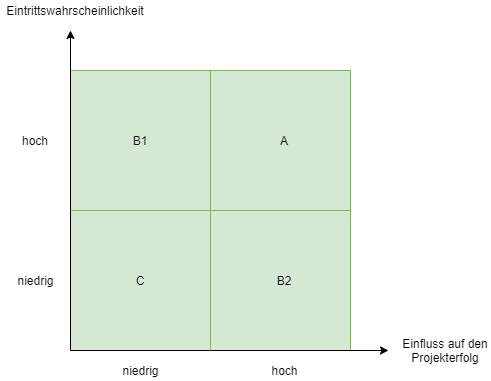
\includegraphics[width=10cm]{4-Felder-Methode.png}
    \caption{4-Felder-Methode (in Anlehnung an die Abbildung im Buch Systemplanung und Projektentwicklung von Felix Schwab und Ingrid Schwab-Matkovits)}
\end{figure}
\end{center}

\begin{itemize}
	\item Bereich A: Hier sind Sofortmaßnahmen durchzuführen, ansonsten könnte es möglicherweise zum Projektende führen.
	\item Bereich B1: Die Risikogestaltung soll mit gewissen Maßnahmen abgewickelt werden.
	\item Bereich B2: Es sollte bei diesem Bereich eine Risikovorsoge mit bestimmten Versicherungen festgelegt werden.
	\item Bereich C: Das sind Risiken die nicht eine hohe Priorisierung benötigen, diese können am Ende von aller Risiken bearbeitet werden\footcite{risikomanagement-diplomarbeit}.
\end{itemize}

%Syp-Buch S.142
\paragraph{Quantitative Methoden}
Mit quantitativen Methoden kann man die Schadenshöhe bei Eintritt eines Ereignisses feststellen. Ein Risiko ist wird hier mit einem Geldwert dargestellt.
Das kann durch die Hilfe des Projektstrukturplans festgestellt werden oder mit beschreibenden statistischen Verfahren\footcite{risikomanagement-diplomarbeit}.

\subsection{Risikogestaltung}
Bei der Risikogestaltung wird vor Eintritt eines Ereignisses Maßnahmen gesetzt, um diese entweder zu verringern oder wenn möglich zu vermeiden.
Es kann bei der Risikogestaltung kann entweder präventiv oder korrektiv vorgegangen werden\footcite{risikomanagement-diplomarbeit}.

%https://www.computerweekly.com/de/definition/Risikovermeidung
\subsubsection{Risikovermeidung}
Dieser Prozess versucht, dass die Firma einem potenziellen Risiko von Vorhinein gar nicht erst ausgesetzt wird. Das kann durch die Erstellung von Richtlinien, Prozeduren und Schulungen gelöst werden\footcite{risikomanagement-diplomarbeit}.

%https://strafrecht-online.org/problemfelder/at/tb/obj-zur/risikoverringerung/
\subsubsection{Risikoverringerung}
Bei diesem Prozess werden die internen- als auch externen Risiken betrachtet. es wird versucht diese abzuschwächen oder zeitlich zu verzögern. Durch die Erstellung von gewissen Gegenmaßnahmen kann dann das Risiko verringert werden\footcite{risikomanagement-diplomarbeit}.

\subsubsection{Risikoüberwälzung}
Hier werden mögliche vertraglich gebundene Verpflichtungen abgeschlossen. Das können z.B. Versicherungen oder Cloud-Services sein. Diese nehmen dem eigenen Unternehmen Risiken ab. Beachtet werden muss das, wenn die eigene Sicherheit verstärkt wird, auch die Kosten dafür steigen. Wichtig zu beachten ist, dass solche Abnehmer nur Risiken übernehmen können, worauf dieser Einfluss haben kann\footcite{risikomanagement-diplomarbeit}.

\subsubsection{Risikoübernahme}
In diesem speziellen Fall geht es um den möglichen Eintritt eines speziellen Risikos. Diese Bedrohung war entweder schon bekannt oder ist vermeintlich unbekannt geblieben. Hier sollten die im Vorhinein geplanten Rücklagen bereitstehen, um solche Risiken aufzufangen\footcite{risikomanagement-diplomarbeit}.

\subsection{Regelmäßige Kontrolle}
Die Liste der Gegenmaßnahmen wird genauso, wie die Risikoliste, sollte regelmäßig aktualisiert werden\footcite{bva-risikomanagement}.  

\section{EMS Risikomanagement}
Im Projekt EMS wurde das Thema Risikomanagement systematisch auf Basis von ISO 27001 beachtet. Dies wurde in der Planungsphase sowie in der Umsetzungsphase als integraler Bestandteil des Projektmanagements betrachtet. Durch regelmäßige Kontrolle und die Sensibilisierung aller Projektmitarbeiter auf den Themenbereich, konnte ein hohes Niveau mit akzeptablen Kosten erreicht werden. Essenziell wird es sein diese Maßnahmen auch im operativen Betrieb weiterzuführen.

\subsection{Verantwortlichkeit und Budgetierung}
Am Beginn des Gesamtprojekts wurde der Projektleiter (Benjamin Strahlhofer) als der Verantwortliche für das Vorhaben Anmeldesysteme festgelegt. Dieser leitete dies bezüglich das Risikomanagement für diese Themenstellung ein.
Da dieses Projekt im Rahmen der Matura umgesetzt wurde, war kein Kostenbudget, sondern ein Zeitbudget von 180 Stunden definiert. Da das Vertrauen des Auftraggebers und der Kunden von EMS wichtig ist wurde ein Hauptaugenmerk darauf gelegt so viele Risiken wie möglich zu bewältigen, um ein mögliches Schadenspotenzial zu minimieren.

\subsection{Risikoidentifizierung}
In der Zeit in dem die Entwicklung des Gesamtprojekt begonnen hat, wurde beraten welche Methoden zur Risikoidentifikation eingesetzt werden. Im Bereich Informationssicherheit konnte erkannt werden, dass durch zwei Hauptmaßnahmen ein großteil der Risiken im Risikomanagement abgedeckt werden können. Dies ist einerseits die Auslagerung des Services in eine Cloud (AWS) und andererseits das Anmeldesystem. Es wurden Vorschläge eingesammelt und als Resultat ergab sich das eine Mindmap eingesetzt wird.
In einem ersten Meeting, das sehr früh in der Planung des Gesamtprojekts stattgefunden hat, wurden mittels Brainstorming die Risiken im Bereich Anmeldesysteme beleuchtet und als komplmentäres Verfahren in einer Mindmap überprüft.

\subsubsection{Brainstorming:}
\begin{center}
\begin{figure}[H]
    \centering
    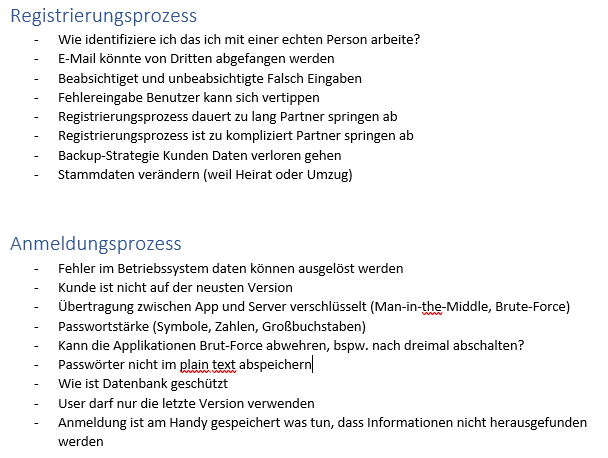
\includegraphics[width=15cm]{brainstorming_risiko_management.PNG}
    \caption{Identifikation von Risiken mittles Brainstorming in einem Anmeldesystem}
\end{figure}
\end{center}

\subsubsection{Mindmap}
Diese Methode wurde im Unterricht den Gruppenmitgliedern beigebracht. Des Weiteren wurde zu der Methode im Vorhinein eine Auffrischung zum Thema Mindmap und Regelungen gemacht.

\subsubsection{Die erstellte Mindmap:}
\begin{center}
\begin{figure}[H]
    \centering
    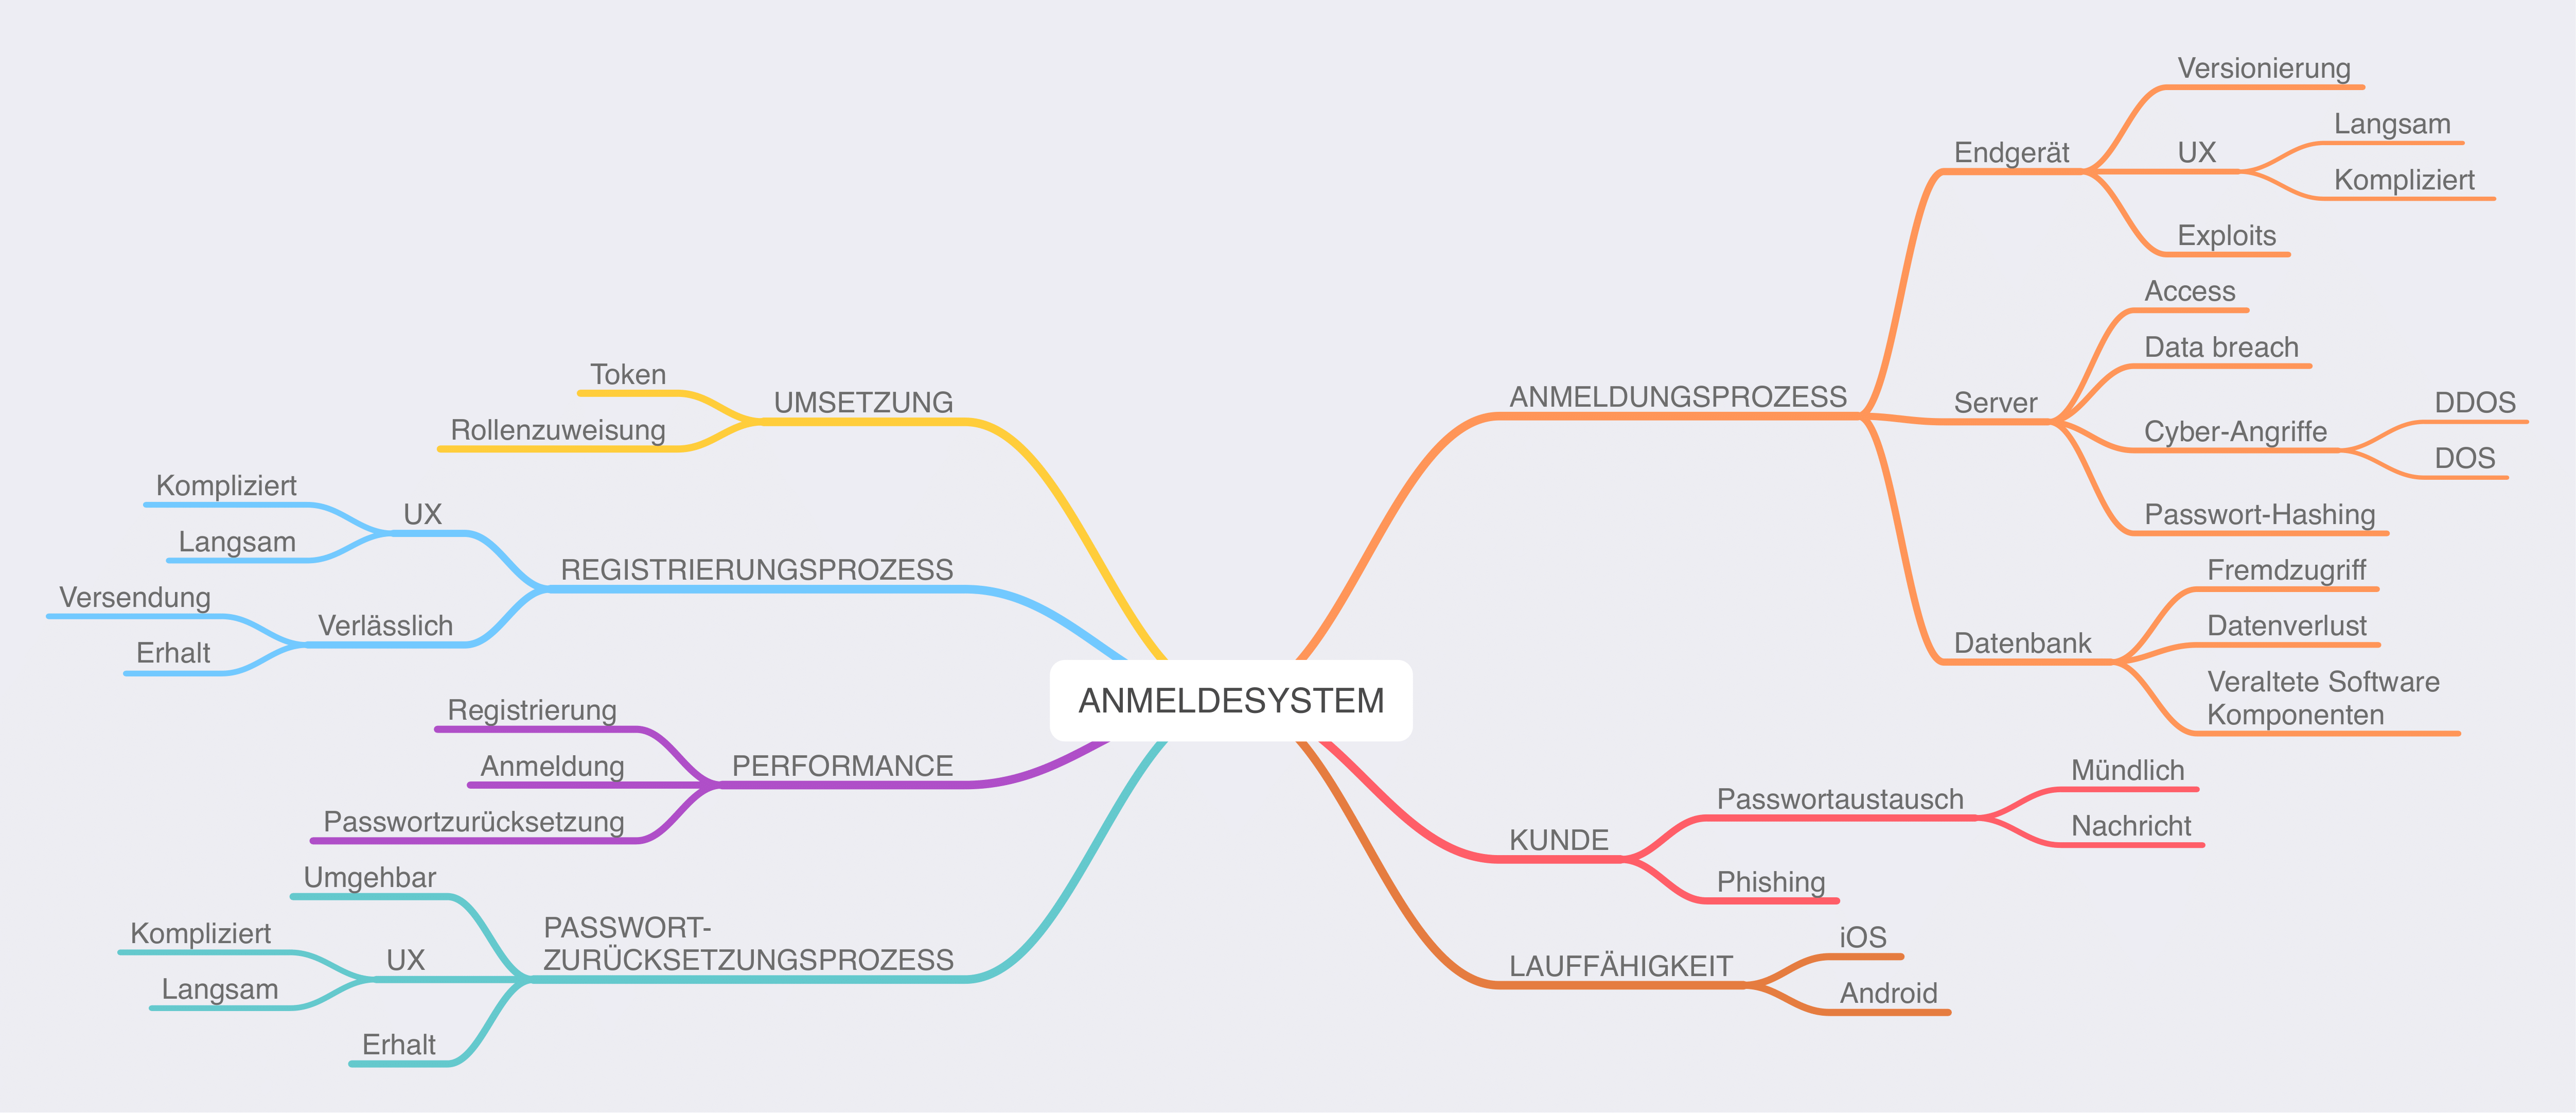
\includegraphics[width=15cm]{mindmap_risiko_management.png}
    \caption{Identifikation von Risiken mittles Mindmap in einem Anmeldesystem}
\end{figure}
\end{center}

\subsection{Umsetzung der Inhalte der Mindmaps}
\subsubsection{Verlässlicher Registrierungsprozess}
Der Registrierungsprozess wurde vom Endnutzer entkoppelt. Der Endnutzer gibt seine Daten per E-Mail ab und die Registrierung am System wird durch einen Administrator durchgeführt. Somit kann das Riskio von Cyberangriffen minimiert werden und die Qualität der eingegeben Daten optimiert werden.
\subsubsection{Rollenkonzept}
Durch das Rollenkonzept wird sichergestellt, dass nur berechtigte Personen Änderungen am System oder den Daten durchführen können. Folgende Rollen und Berechtiungen wurden definert: 
\begin{itemize}
	\item \textbf{Administratoren:} Der Administator kann Benutzer und Events im System erstellen, verändern und löschen. Benutzer können zusätzlich deaktiviert werden, da diese entweder zu häufig falsche Anmeldeinformationen eingegeben haben oder weil die Person eine Anfrage daraufgestellt hat.
	\item \textbf{Promoter:} Diese Rolle sind die Benutzer der Software, die Karten anfordern und verkaufen können. Es wird ebenfalls sichergestellt, dass die Promoter nur Zugriff auf von ihnen erstellte Geschäftsfälle haben.
\end{itemize}

\subsubsection{Passwortzurücksetzungsprozess}
Es ist sichergestellt, dass nur der User sein Passwort vergeben kann. Hat er dieses vergessen, kann er mit der Eingabe seiner E-Mail-Adresse (diese muss mit der Adresse in seinen Stammdaten zusammenpassen) einen Token anfordern. Mit Eingabe des Tokens wird die Identität verifiziert und der User kann ein neues Passwort vergeben.
\subsubsection{Anmeldeprozess}
Durch Verifikation des Users per Username und Passwort authentifiziert der Anwender sich im System. Hierbei wurde noch die Möglichkeit eines Single-Sign-On implementiert in der User durch einen vom System vergebenen Token identifiziert wird. Um das Risiko von Brute-Force oder DoS/DDoS Angriffen zu minimieren wurde zum einen die Passwortsicherheit durch die Vorgabe von Minimalattributen (Mindestens 8 Zeichen, alphanumerisch, Numerisch und Sonderzeichen) sichergestellt. Zum Weiteren wird der Anmeldeversuch nach dem 5 Mal abgebrochen und der User muss durch einen Administrator wieder aktiviert werden.
\subsubsection{Lauffähigkeit}
Durch die Verwendung des Ionic Frameworks wird die Lauffähigkeit auf Android und iOS Systemen sichergestellt.
\subsubsection{Phising}
Die User werden darauf aufmerksam gemacht, dass nur von einer Stelle Nachrichten an sie versendet werden. 
\subsubsection{Passworthashing}
Im System werden alle Passwörter per Geheimschlüssel verschlüsselt verarbeitet und gespeichert.
\subsubsection{Performance}
Bei der Programmierung wurde darauf geachtet nur die notwendigsten Datenmengen zu übertragen. Bei manuellen Tests wurde die Performance entsprechend überprüft. Das Budget lässt keine automatisierten Performance Tests im Projekt zu.
\subsubsection{Durch AWS abgedeckte Risiken}
Risiken wie Datenverlust, veraltete Softwarekomponenten und auch zum Teil DoS/DDoS Angriffe werden durch die Verwendung des Cloud-Dienstes AWS ausgeschlossen oder zumindest verringert.